\paragraph{} Three core questions hang over \textsc{Citadel}'s viability --- its security, expressivity, and performance. This chapter presents a thorough investigation of the prototype's performance profile, a discussion around its security implications, and an illustrative example in favour of its expressability.

\section{Performance}
\label{sec:performance}

\paragraph{} The \textsc{Citadel} prototype demonstrates highly impressive performance, matching, and in places surpassing, related approaches, despite the architectural disadvantage it is at. We present its behaviour relative to native Linux kernel in three ways;

\begin{enumerate}
    \item Application-level microbenchmarks, tracing the duration of \textit{syscalls} both natively and through \texttt{libcitadel}. (§~\ref{sec:syscall-microbenchmarks})
    \item IPC bandwidth microbenchmarks in both \textit{intra-} and \textit{inter-}process contexts. (§~\ref{sec:ipc-microbenchmarks})
    \item Real-world \textsc{Nginx} performance benchmarks for both low-latency and high-bandwidth configurations. (§~\ref{sec:nginx-benchmarks})
\end{enumerate}

\paragraph{}The results presented here are best compared to \textit{Flume}~\cite{flume} --- \textit{CamFlow}, although implemented similarly, has a far greater scope that this project.

\subsection{Evaluation Environment}
\paragraph{} The research machine used for evaluation contained a quad-core Intel® Core™ i5-6600 (which supports SGX v1), 16 GiB RAM, and a 1-Gbps NIC. The primary disk provided 389 MBps read and 210 MBps write.\footnote{As reported by the \texttt{dd} tool.} For all experiments running under \textsc{Citadel}, \texttt{citadeld} was running via \texttt{systemd} --- all debugging tools were disabled and the enclave was built in hardware pre-release mode. Linux v5.6.0 was the base kernel for all trials; \textsc{Citadel} adds its LSM on top of this.

\paragraph{} Both Tables~\ref{table:syscall-microbenchmarks} and \ref{table:nginx-benchmarks} report the sample mean and standard deviation. Figures~\ref{fig:io-graph}, \ref{fig:ipc-2thread-graph}, and \ref{fig:ipc-2proc-graph} plot the sample medians and interquartile range for each point. The Wilcoxon paired signed rank test was chosen to determine statistical significance.~\cite{10.2307/3001968}

\subsection{\textit{syscall} Microbenchmarks}
\label{sec:syscall-microbenchmarks}

\begin{figure}[]
    \centering
    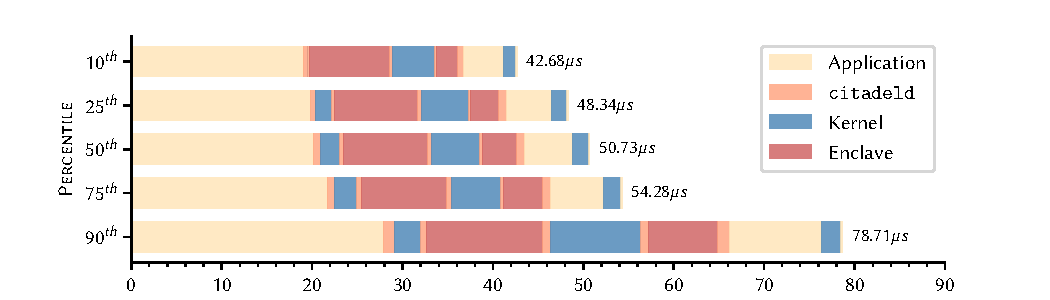
\includegraphics[width=\linewidth]{figures/graphs/open-anatomy.pdf}
    \vspace{-5mm}
    \caption{Control flow inhabitation for \texttt{libcitadel}'s \texttt{c\_open()} function, $n=100$.}
    \label{fig:open-anatomy}
\end{figure}


\begin{table}
    \centering
    \newcommand\tableTop{\rule{0pt}{3ex}}
    \newcommand\tableMid{\rule{0pt}{3ex}}
    \newcommand\tableBottom{\rule[-2ex]{0pt}{0pt}}
    \newcolumntype{N}{>{\centering\arraybackslash}m{2.5in}}
    
    \renewcommand\theadfont{\normalsize}
    \renewcommand\arraystretch{1.3}
    \begin{tabular}{l@{\hskip 0.15in} r@{\hskip 0.6in} r@{\hskip 0.35in} r} 
        
        \toprule
        & \thead{\multirow{2}{*}{\textsc{Native}}} & \multicolumn{2}{c}{\thead{\textsc{Citadel}}} \\
        \cline{3-4}
        &  & \thead{\textit{Amortised}} & \thead{\textit{Cache Miss}} \\
        % \cline{1-4}
        \midrule 
        \texttt{open()} & $1.675\pm0.076$ & $6.083\pm0.129$ & $50.133\pm1.482$ \\
        \texttt{read()} & $5.724\pm0.206$ & $7.010\pm0.192$ & $54.736\pm1.556$ \\
        \texttt{write()} & $14.340\pm0.208$ & $15.597\pm0.250$ & $63.824\pm1.902$ \\
        \texttt{close()} & $0.651\pm0.005$ & \multicolumn{2}{c}{$0.718\pm0.011$} \\

        

        \midrule 
        \texttt{socket()} & $1.446\pm0.179$ & \multicolumn{2}{c}{$3.156\pm0.291$} \\
        \texttt{bind()} & $0.762\pm0.023$ & $1.911\pm0.183$ & $49.110\pm1.746$ \\
        \texttt{listen()} & $0.705\pm0.015$ & $1.882\pm0.149$ & $48.411\pm1.386$ \\
        \texttt{connect()} & $16.570\pm0.278$ & $17.961\pm0.330$ & $66.273\pm2.147$ \\

        \midrule 
        \texttt{shmget()} & $1.880\pm0.122$ & $1.913\pm0.111$ & $49.326\pm1.466$ \\
        \texttt{shmat()} & $0.420\pm0.005$ & $1.575\pm0.134$ & $47.997\pm1.560$ \\
        \texttt{shmctl()} & $0.418\pm0.005$ & $0.743\pm0.083$ & $45.912\pm1.114$ \\
        \texttt{shmdt()} & $0.415\pm0.003$ & \multicolumn{2}{c}{$1.342\pm0.040$} \\



        \midrule 
        \texttt{pipe()} & $1.110\pm0.061$ & $1.288\pm0.069$ & $47.334\pm1.147$ \\
        \texttt{mkfifo()} & $3.865\pm0.048$ & $11.509\pm0.405$ & $59.623\pm1.788$ \\

        \midrule 
        \texttt{fork()} & $47.866\pm3.175$ & $48.647\pm3.457$ & $81.174\pm3.829$ \\
        \texttt{citadel\_init()} & $-$ & $0.801\pm0.009$ & $34.940\pm1.329$ \\
        \bottomrule
    \end{tabular}
    \vspace{5mm}
    \captionsetup{justification=centering}
    \caption[\texttt{libcitadel} microbenchmarks]{\texttt{libcitadel} microbenchmarks. \\ All values are in $\mu s$ and the sample standard deviation is shown alongside the mean. For \textsc{Citadel}, both the amortised and average cache-miss durations are given. Only one value is given if the operation is not affected by a cache miss. $n=10^6$.}
    \label{table:syscall-microbenchmarks}
\end{table}

\begin{figure}[h]
    \centering
    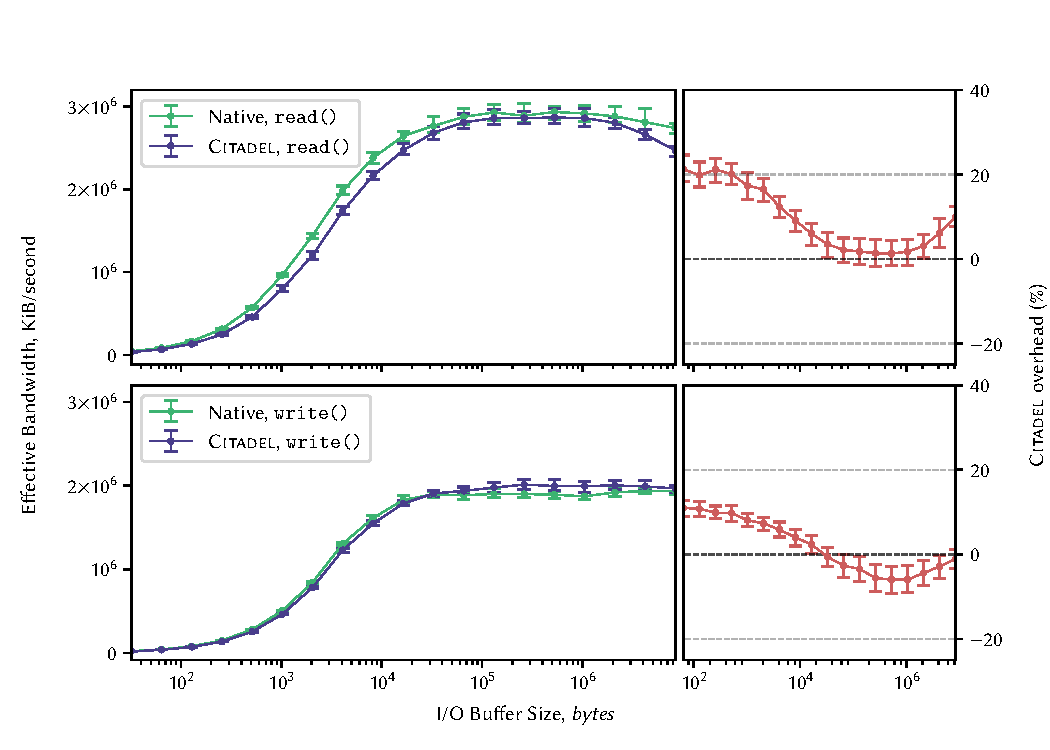
\includegraphics[width=\linewidth]{figures/graphs/io.pdf}
    \vspace{-5mm}
    \captionsetup{justification=centering}
    \caption[Effective \texttt{read()/write()} bandwidths for both the native Linux kernel and \textsc{Citadel}.]{Effective \texttt{read()/write()} bandwidths for both the native Linux kernel and \textsc{Citadel}. The percentage overhead is also presented. $n=200$ per buffer size.}
    \label{fig:io-graph}
\end{figure}

\paragraph{} A custom benchmark tool was built to assess the overall impact \textsc{Citadel} has on \textit{syscall} performance --- for example, the duration of \texttt{open()} compared to \texttt{c\_open()}. Table~\ref{table:syscall-microbenchmarks} presents these results. To give a fair comparison, two figures are reported for \textsc{Citadel}. \textit{Amortised} refers to the normal operation of \texttt{libcitadel}, in which the majority of queries are served from the cache; overhead arises from both local cache operations and added kernel latency from the LSM. The other figure, \textit{Cache Miss}, gives the overhead when caching is disabled, thus including communication with \texttt{citadeld}.

\paragraph{} Overall \texttt{libcitadel} contributes $\sim{}1 \mu s$ of overhead (amortised) on average --- this rises to $\sim$~$40 \mu s$ on a cache miss. Figure~\ref{fig:open-anatomy} presents a more detailed view of where exactly this overhead arises, approximately plotting where the control flow for \texttt{c\_open()} moves (on a cache miss). Interestingly, the slowest component is the communication channel between \texttt{libcitadel} and \texttt{citadeld} ($26\mu s$ median);\footnote{Included in the \textit{Application} regions.} as a result, the core reference monitor functionality only adds a median penalty of $24\mu s$. The final \textit{Kernel} call before terminating is the internal call to \texttt{open()}. Additionally, the $10^{th}$ percentile demonstrates that the first \textit{Kernel} call is not always required if the entity's metadata is resident in the cache.

\paragraph{} Figure~\ref{fig:io-graph} plots observed effective bandwidth whilst reading from and writing to a 16 MiB file with different sized buffers. The benchmark driving this was adapted for Linux from one written by R.~Watson for FreeBSD.~\cite{l41-benchmark} The results clearly show \textsc{Citadel} having a more adverse effect on performance for smaller buffer sizes; this is logical, as smaller buffers force a larger number of calls to \texttt{read()}/\texttt{write()}. The reason for \textsc{Citadel} providing better performance for large buffers with \texttt{write()} is unclear --- the difference is statistically significant (at 5\% confidence) and reproducable. More work is required to 
narrow down the root causes, but hypotheses include the fact that regular, small delays could ease pressure on microarchitectural cache in the processor, affording slight optimisations.



\subsection{IPC Microbenchmarks}
\label{sec:ipc-microbenchmarks}

\paragraph{} Again using the modified Watson benchmark, we investigated the effect \textsc{Citadel} has on end-to-end IPC performance. We investigate \textit{pipes}, \textit{local sockets} (\texttt{socketpair()}), and \textit{regular sockets}, between 2 threads (Figure~\ref{fig:ipc-2thread-graph}) and between a parent and child process (Figure~\ref{fig:ipc-2proc-graph}).

\paragraph{} Overall the results between the two contexts are similar --- both see approximately 20\% degradation in the worst cases, tending towards equal performance when using $\sim 10^5$-byte blocks. At first glance it would appear that \textsc{Citadel} affects the performance between 2 threads slightly more than 2 processes, but in fact the truth is that \textsc{Citadel} performs nearly identically in both. The native performance is more heavily optimised when sending between two threads; any latency gained by the kernel is overshadowed by \textsc{Citadel}.

\paragraph{} In a similar way to \texttt{write()}, \textsc{Citadel} outperforms the native kernel in both contexts using \texttt{pipe()}. The readings are noisy, but statistically significant (at 5\%) and reproducable. The causes is again unknown, but noting that the native kernel's throughput halves after buffers of 8 KiB, we highly suspect that this is the result of cache exhaustion or inopportune paging. It is also notable that readings for \textsc{Citadel} exhibit a far larger interquartile range for large buffer sizes than the native kernel, a side effect that we see repeated in real-world testing.

\begin{figure}[]
    \centering
    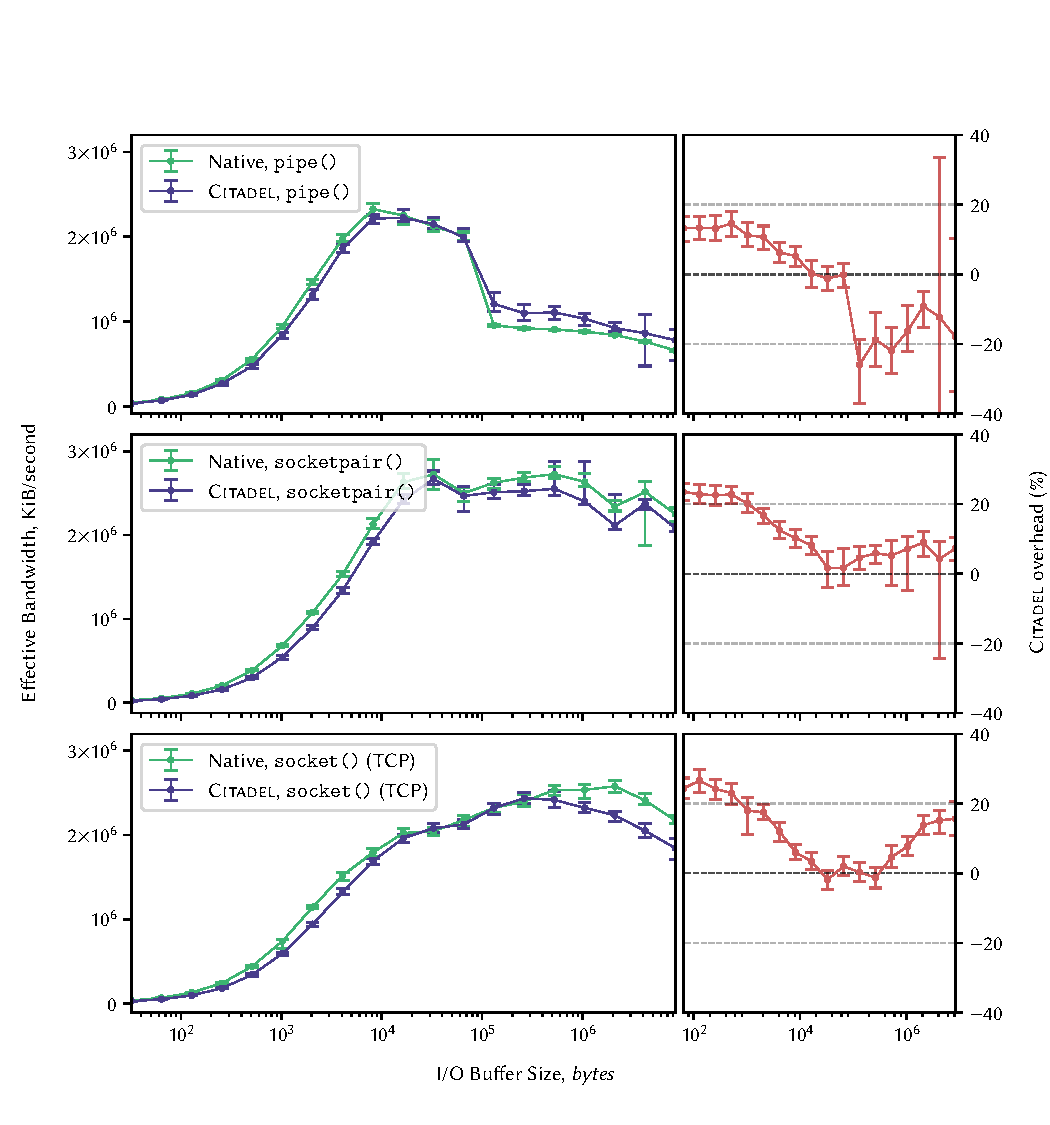
\includegraphics[width=\linewidth]{figures/graphs/ipc-2thread.pdf}
    \vspace{-5mm}
    \caption{Effective bandwidths for various types of IPC between \textit{2 threads}, $n=200$.}
    \label{fig:ipc-2thread-graph}
\end{figure}


\begin{figure}[]
    \centering
    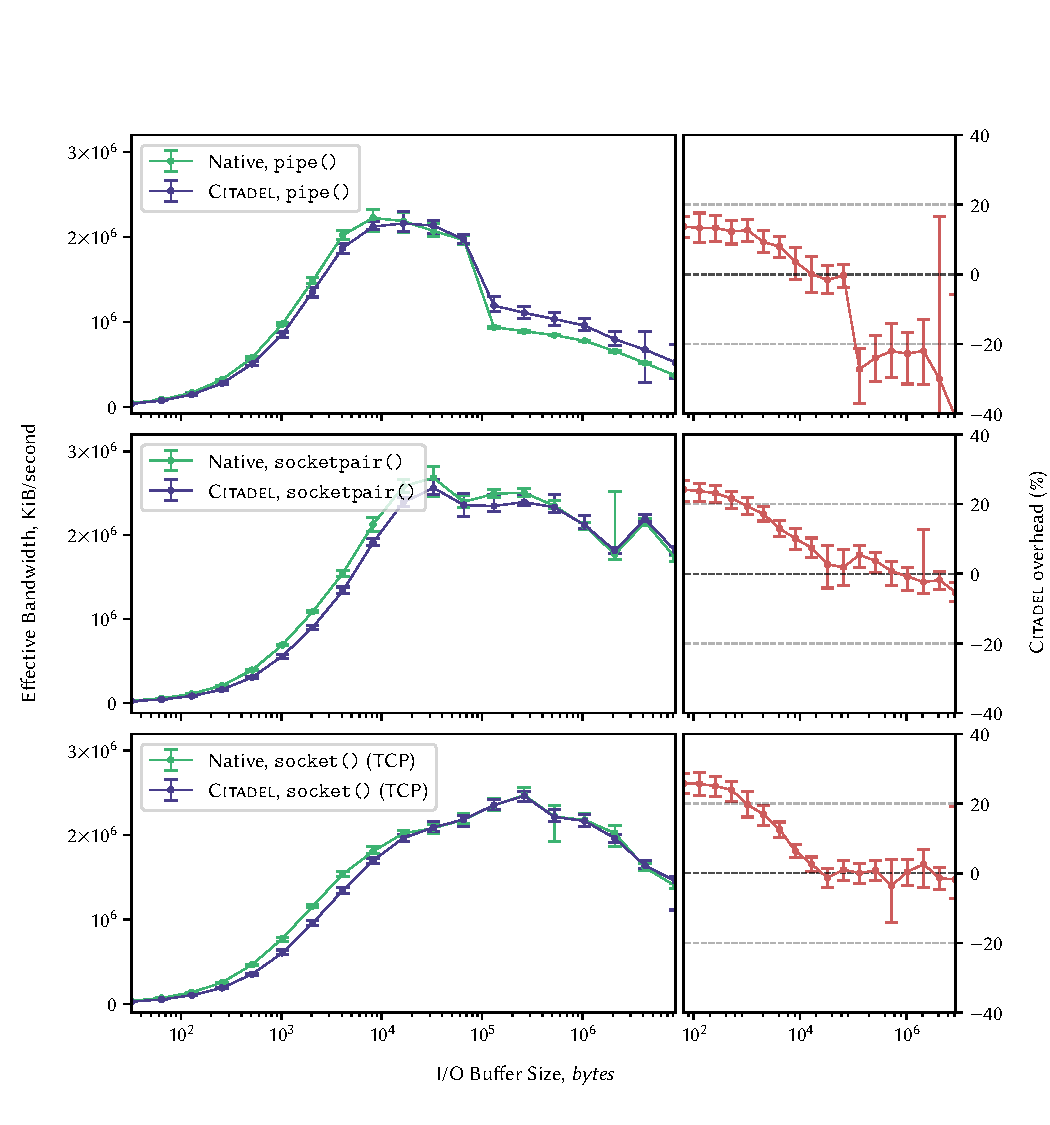
\includegraphics[width=\linewidth]{figures/graphs/ipc-2proc.pdf}
    \vspace{-5mm}
    \caption{Effective bandwidths for various types of IPC between \textit{2 processes}, $n=200$.}
    \label{fig:ipc-2proc-graph}
\end{figure}

\clearpage

\subsection{\textsc{Nginx} Benchmarks}
\label{sec:nginx-benchmarks}
\begin{table}
    \centering
    \newcommand\tableTop{\rule{0pt}{3ex}}
    \newcommand\tableMid{\rule{0pt}{3ex}}
    \newcommand\tableBottom{\rule[-2ex]{0pt}{0pt}}
    \newcolumntype{N}{>{\centering\arraybackslash}m{2.5in}}
    
    \renewcommand\theadfont{\normalsize}
    \renewcommand\arraystretch{1.3}
    \begin{tabular}{l@{\hskip 0.35in} r@{\hskip 0.3in} r@{\hskip 0.35in} r@{\hskip 0.35in} c} 
        
        \toprule
        & \thead{\multirow{2}{*}{\textsc{Native}}} & \multicolumn{3}{c}{\thead{\textsc{Citadel}}} \\
        \cline{3-5}
        &  & \thead{\textit{Untainted}} & \thead{\textit{Tainted}} & \thead{\textit{Overhead}} \\
        % \cline{1-4}
        \midrule 
        \multicolumn{5}{l}{\textsc{Webserver Benchmark}, \textit{100-byte packets}} \\
        \textit{Latency} & $35.73\mu s$ & $36.18\mu s$ & $44.35\mu s$ & $24\%$ \\
        $-\;$ \textit{std. dev.} & $13.85\mu s$ & $14.12\mu s$ & $13.26\mu s$ & \\
        $-\;$ \textit{max.} & $536\mu s$ & $554\mu s$ & $508\mu s$ & \\
        \textit{Requests/s} & $2.748 \cdot 10^4$ & $2.717 \cdot 10^4$ & $2.214 \cdot 10^4$ & $19\%$\\
        \textit{Bandwidth} & $177.28$ Mbps & $168.72$ Mbps & $143.04$ Mbps & $18\%$\\

        \midrule 
        \multicolumn{5}{l}{\textsc{10GB File Transfer}} \\
        \textit{Bandwidth} & $1.404$ Gbps & $1.410$ Gbps & $1.413$ Gbps & $\sim 0\%$ \\
        $-\;$ \textit{std. dev.} & $0.428$ Gbps & $0.440$ Gbps & $0.549$ Gbps &\\
        \textit{Duration} & $56.98 s$ & $56.74 s$ & $56.62 s$ & $\sim 0\%$ \\
        $-\;$ \textit{std. dev.} & $19.45 s$ & $18.97 s$ & $23.63 s$ & \\
        
        \bottomrule
    \end{tabular}

    \vspace{5mm}
    \captionsetup{justification=centering}
    \caption{\textsc{Nginx} performance comparinson between native Linux, and both untainted and tainted \textsc{Citadel}, $n=25$.}
    \label{table:nginx-benchmarks}
\end{table}

\paragraph{} To validate the performance results presented thusfar, we ported the entirety of the \textsc{Nginx} webserver\footnote{\url{https://www.nginx.com/}} to function inside \textsc{Citadel}. No optimisations were made to the codebase --- the only changes were changing core \texttt{libc} function calls to use their \texttt{c\_*} \texttt{libcitadel} counterpart.

\paragraph{} Two trials were run; a low-latency benchmark\footnote{\url{https://github.com/wg/wrk}} and a 10GB HTTP file transfer (high-bandwidth). The webserver was configured to only run a single server process to ensure it was exercised to its full extent, and was setup to use the \textit{loopback} interface\footnote{\texttt{http://127.0.0.1/}.} to eliminate any interference from outside the OS. 

\paragraph{} The results, displayed in Table~\ref{table:nginx-benchmarks}, are not suprising. For the low latency tests we observe the same 20-25\% overhead as seen from TCP sockets in §~\ref{sec:ipc-microbenchmarks} using the same buffer size. The high-bandwidth tests show \textsc{Citadel} performing equally as the native kernel, only differing in that it had a larger sample standard deviation. The large file transfer is also interesting as it is the first time we see file descriptor revalidation happening automatically in the wild on \texttt{read()} and \texttt{write()} being called. 
